\documentclass[output=paper]{../langscibook}
\author{Barbara Hofer\affiliation{Dyme Research Group, Innsbruck University}}
\title{Exploring learner attitudes in multilingual contexts: An empirical investigation at the primary school level}
\abstract{Recent research highlights the dynamic and complex nature and the situatedness of multilingual development. It emphasises the need for learners to have ample opportunity for interaction in order to progress on their learning trajectories and suggests that positive attitudes and emotions are key to language learning motivation and learning outcomes. Indications are that how children feel about languages and language learning can impact their learning behavior and willingness to engage with a particular L2/Ln. In this paper I investigate how sociolinguistic and educational context and amount of contact with the L2 (and/or other languages) relate to learner attitudes at the primary level. I report on work in progress carried out in variously multilingual settings in South Tyrol with the aim of establishing whether learning in multilingual contexts as opposed to monolingual surroundings has any effect on pupils’ attitudes and motivations. To my knowledge no previous studies in South Tyrol have looked into attitudinal factors and/or young learners’ beliefs with regards to language(s). The present research seeks to bridge this gap.}
\IfFileExists{../localcommands.tex}{
  \addbibresource{../localbibliography.bib}
  % add all extra packages you need to load to this file

\usepackage{tabularx,multicol}
\usepackage{url}
\urlstyle{same}

\usepackage{enumitem}

\usepackage{pifont}

\usepackage{listings}
\lstset{basicstyle=\ttfamily,tabsize=2,breaklines=true}

\usepackage{./langsci-optional}
\usepackage{./langsci-lgr}
\usepackage{./langsci-gb4e}

\usepackage{langsci-plots} 

\makeatletter
\let\pgfmathModX=\pgfmathMod@
\usepackage{pgfplots,pgfplotstable}%
\let\pgfmathMod@=\pgfmathModX
\makeatother

\usepackage{siunitx}
\sisetup{output-decimal-marker={.},detect-weight=true, detect-family=true, detect-all, input-symbols={\%}, free-standing-units,table-align-text-pre=false,group-digits=false,detect-inline-weight=math}
\DeclareSIUnit[number-unit-product={}]{\percent}{\%}
\makeatletter \def\new@fontshape{} \makeatother
\robustify\bfseries % For detect weight to work

\usepackage{todonotes}

  \newcommand*{\orcid}{}

\renewcommand{\lsChapterFooterSize}{\footnotesize}

\makeatletter
\let\thetitle\@title
\let\theauthor\@author
\makeatother

\newcommand{\togglepaper}[1][0]{
%   \bibliography{../localbibliography}
  \papernote{\scriptsize\normalfont
    \theauthor.
    \thetitle.
    To appear in:
    Jorge Pinto \& Nélia Alexandre (eds.),
    Multilingualism and third language acquisition: Learning and teaching trends.
    Berlin: Language Science Press. [preliminary page numbering]
    }
  \pagenumbering{roman}
  \setcounter{chapter}{#1}
  \addtocounter{chapter}{-1}
}


 
  %% hyphenation points for line breaks
%% Normally, automatic hyphenation in LaTeX is very good
%% If a word is mis-hyphenated, add it to this file
%%
%% add information to TeX file before \begin{document} with:
%% %% hyphenation points for line breaks
%% Normally, automatic hyphenation in LaTeX is very good
%% If a word is mis-hyphenated, add it to this file
%%
%% add information to TeX file before \begin{document} with:
%% %% hyphenation points for line breaks
%% Normally, automatic hyphenation in LaTeX is very good
%% If a word is mis-hyphenated, add it to this file
%%
%% add information to TeX file before \begin{document} with:
%% \include{localhyphenation}
\hyphenation{
affri-ca-te
affri-ca-tes
au-ton-o-mous
Cha-basse
Din-ger-fel-der
plu-ri-lin-gual
Ya-na-pra-sart
Mi-ri-ci
Ström-quist
}

\hyphenation{
affri-ca-te
affri-ca-tes
au-ton-o-mous
Cha-basse
Din-ger-fel-der
plu-ri-lin-gual
Ya-na-pra-sart
Mi-ri-ci
Ström-quist
}

\hyphenation{
affri-ca-te
affri-ca-tes
au-ton-o-mous
Cha-basse
Din-ger-fel-der
plu-ri-lin-gual
Ya-na-pra-sart
Mi-ri-ci
Ström-quist
}
 
  \togglepaper[1]%%chapternumber
}{}

\shorttitlerunninghead{Exploring learner attitudes in multilingual contexts}
\begin{document}
\maketitle 
\shorttitlerunninghead{Exploring learner attitudes in multilingual contexts}



% \begin{stylelsAbstract}
% Keywords: early multilingual learning, learner attitudes, multilingual contexts, DMM, complexity, (dynamic) systems thinking. 
% \end{stylelsAbstract}


\section{Introduction}

International research has found that the way children feel about languages and language learning can impact their learning behavior and willingness to engage. No previous studies carried out in South Tyrol that I know of, have looked into young learners’ (YLs) attitudes and/or beliefs relative to language(s) and language learning. The present study therefore sets out to fill this gap by probing into primary schoolers’ language-related attitudes and motivations. 

I begin by outlining the epistemological framework within which this research is situated linking it to related theoretical perspectives, which converge on the importance of context for multilingual growth and point to the interconnectedness of cognitive activity, psychological constructs and contextual circumstances. I then provide a cursory overview of research into contextual matters and learner attitudes and examine how they may be linked to multilingual development. Next, I present the study, mapping out the aims and research question and the sociopolitical and -linguistic background in which the research is embedded. Finally, I report on selective quantitative and qualitative findings and discuss them within a dynamic systems and complexity theory frame of reference. The paper closes with implications for educational practice in South Tyrol and offers recommendations for future research.


\section{A DMM perspective on multiple language development}


The present research is informed by the \emph{dynamic model of multilingualism} (DMM, \citealt{HerdinaJessner2002}). DMM is widely acknowledged as a valid explanatory framework for the complex dynamics involved in multilingual development. The model has been credited for making significant contributions to current understandings of multilingualism and multilingual acquisition. Positing the total interconnectedness of the cognitive, psychological, social, cultural and physical, DMM focuses on the multilingual speaker as highly complex and adaptive systems in constant interaction with their environments. 

From a DMM perspective, multilingual growth or development are seen as conditional on learner-users’ perceived needs and motivations, and on GLE (General Language Effort, \citealt{HerdinaJessner2002}: 131). GLE relates to the amount of effort individuals are willing to expend in order to learn a language (Language Acquisition Effort, LAE) and to the amount of effort they invest in the maintenance of their languages (Language Maintenance Effort, LME). 

DMM anticipates multilingual learner-users to benefit from a so-called multilingualism factor (M-factor) which mitigates the amount of GLE needed to learn and maintain a given L2/Ln (Ln denoting any language beyond the speaker’s second language) and affords them enhanced possibilities for action.  Endowing the system with special qualities, the M-factor comprises a range of skills and abilities which multilinguals develop as a function of the dynamic interactions between their multiple languages including language learning, language management and language maintenance skills, an Enhanced Multilingual Monitor (EMM), and enhanced Meta- and Crosslinguistic Abilities (MLA and XLA). Key components of the M-factor, meta- and crosslinguistic abilities are the most distinguishing features of the multilingual system (\citealt{JessnerEtAl2018}). 

Grounded in dynamic systems theory, DMM embraces the idea of holism, which entails a global, holistic approach to multilingual phenomena. Holistic paradigms are characterised by a conception of the multilingual learner-user as an integrated and complete whole, and as constituted by their relationship to other systems \citep[44]{Philips2000}, in other words, nested in a greater whole and continuously interacting with its surroundings. 

It is against this backdrop of total interconnectedness that DMM posits the need to integrate the psycholinguistic with a sociolinguistic focus in order to take adequate account of the complexities of multilingual learning and use. Starting from the premise that “[l]inguistic aspects of individual multilingualism are shaped by the sociolinguistic setting in which the multilingual’s life takes place” \citep[273]{Jessner2008}, the implication is that the multilingual system is molded as much by social factors as by “individual cognitive factors such as motivation, anxiety, language aptitude, and self-esteem” \citep[274]{Jessner2008}. 

The situatedness of multilingual development is also highlighted in complexity theory-inspired and ecological approaches to applied linguistics (e.g. \citealt{Kramsch2012,Larsen-FreemanCameron2008,LaoireAronin2004}), which point to social and cultural settings as crucial factors contributing to the individual’s multilinguality. In consonance with DMM, complexity and ecological thinking endorse a view of multilingual agency and subjectivity as resulting from complex and dynamic interactions taking place on different levels and timescales, and thence as multifaceted and multi-layered, rather than self-contained and reducible to single causes.


In the following I discuss core principles underlying these paradigms and I examine how they tie in with the DMM perspective and the exploratory foci of the present study.

\section{Complexity theory and ecological approaches}

Complexity theory (henceforth CT) implicates thinking in terms of connectedness, relationships and context. It is premised on the recognition that “all natural phenomena are ultimately interconnected, and that their essential properties, in fact, derive from their relationships to other things” (\citealt{CapraLuisi2018}: 2). Accordingly, CT conceives of individual learner-users as open systems who interact with and (if necessary) adapt to multiple contextual factors in time and space (cf. \citealt{HerdinaJessner2002}). Context as an intrinsic part of the system rather than merely “background against which action takes place” (\citealt{Larsen-FreemanCameron2008}: 16) is seen as playing an all-important role with the individual and her/his context subsisting in a relationship of “reciprocal causality” (\citealt{Larsen-FreemanCameron2008}: 7). The present research dovetails with this line of thinking as it explores the complex associations between contextual factors and learner attitudes.

By the same token, ecological perspectives predicated on the understanding that systems “are bound into a functional whole by their mutual relationships” (\citealt{CapraLuisi2018}: 67) impel acknowledgement “of the interconnectedness of individuals, pairs of individuals, communities, etc.” (\citealt{Larsen-FreemanCameron2008}: 19). It is this interconnectedness and reciprocity that \citet[19]{KramschSteffensen2008} invoke when they posit that it is in contact situations (or dialogue, to use the authors’ wording) that the personal, situational, and cultural merge, and interaction obtains affording learners the possibility to develop and grow. As for the current investigation, the aim is to ascertain whether different sociolinguistic ecologies and contact opportunities as provided by learner-users’ everyday life realities affect their attitudes towards languages and language(s) learning.

\section{Multilingual learning context}

Highlighting the importance of context, \citet[203]{BlommaertEtAl2005} argue that context is crucial because it “does something to people” and in so doing influences “what people can do and can become” (cf. \citealt{Cenoz2013Influence}: 79; \citealt{VanGeertEtAl2011}: 240). Investigating learner attitudes in Sweden, \citet[611]{HenryApelgren2008} confirm that there is substantial interindividual variation depending on the cultural context in which learning takes place. It then seems that if we are to understand the multilingual learner-user system better, we need to take adequate account of the larger context in which the system operates (\citealt{Larsen-FreemanCameron2008}: 35; \citealt{PaladinoVaes2009}: 223). 

In the present study, context understood as the here and now in which a system is active (\citealt{ThelenSmith1994}: 217) relates in particular to different sociolinguistic and educational settings which range from the relatively monolingual to the highly multilingual. I delineate these settings in some detail in the second part of the paper. Here, I discuss possible associations between contact with the target language community on the one hand and multilingual growth and learner attitudes on the other.

Discussing language (learning) in terms of situated practice and as requiring “participation in […] communities of practice” Blommaert et al. (\citeyear[206]{BlommaertEtAl2005}; cf. \citealt[81]{Cenoz2013Influence}) imply that participation in a given L2/Ln community of practice is conditional on the sociolinguistic context, viz., the linguistic demographics and the presence of other-language speakers in the immediate surroundings. This is supported by empirical evidence which suggests that increased contact time with L2/Ln speakers creates favourable conditions for learning because it provides important opportunities for learners to communicate (\citealt{DeAngelis2012}: 408; see also \citealt{Kordt2018}) and thus acts as a catalyst for language(s) learning (cf. \citealt{Bozzo2014}). Investigating the effects of population distribution on L1 and L2 acquisition in South Tyrol, De Angelis, for instance, found that opportunity to communicate in L2 is highly beneficial for acquisition (\citealt{DeAngelis2012}: 420; see also \citealt{DeAngelisNodate}). Along similar lines, \citet[63]{CsizerKormos2009} argue that interaction with speakers of other languages creates important opportunities for developing L2 learners’ language competence. In the DMM, acknowledgement of the centrality of contact with L2/Ln (speakers) is reflected in the postulate that regular use of the target language(s) is vital for the maintenance of both the single languages, and the overall multilingual system (\citealt{HerdinaJessner2002}: 99; see also \citealt[158]{Schmid2011} on the importance of contact and frequency of use for language maintenance).

The paper now moves on to consider the effects of affective and attitudinal factors on multilingual development.

\section{Learner attitudes and multilingual growth}


Attitudes have been variously described as evaluative orientations to a given social object or phenomenon (\citealt{Garret2010}; \citealt{Cenoz2004}), and as sets of beliefs and psychological predispositions (\citealt[124]{TodorDegi2016}). 

Research into young learners’ language-related attitudes has shown that, from a very young age, children form views and hold beliefs about languages and language(s) learning \citep{Munoz2014,NagyNikolov2009,Nikolov2009}. As is well-documented, learner attitudes and language-related emotions have a significant role to play in second and foreign language learning (\citealt[3]{CourtneyEtAl2017}; \citealt[58]{Culhane2004}; Portolés \citealt[77]{Falomir2015}). The understanding is that affective and attitudinal factors are closely linked to learner efficiency, self-concept and learning success (\citealt{DornyeiEtAl2015}; \citealt[197]{MacIntyreGregersen2012}; \citealt{MacintyreEtAl2016}; \citealt{Wesely2012}). In like manner, there is general agreement that positive attitudes towards a language and/or its speakers will result in enhanced levels of motivation, increase learners’ readiness to engage and contribute to higher overall attainment (\citealt{MacIntyreGregersen2012}: 193).

Primary schoolers seem to be particularly influenced by what goes on in the second or foreign language classroom with teachers, methodology, classroom activities, and overall learning atmosphere all contributing to shaping their orientations towards a particular language and towards language(s) learning in general \citep{Nikolov1999}. Research reported by \citet[155]{Chambers1999} found that 12 to 14-year-olds’ attitudes towards learning English declined as a result of classroom approaches and teaching methodology that failed to match their expectations. On a related note, \citet[107]{Wesely2012} suggests that young learners’ perception of the classroom setting and teaching methodology can have a lasting impact with early language learning experiences at the primary level potentially persisting with learners and influencing their attitudes far into adulthood. Likewise, parents act as important models (\citealt[205]{Cenoz2004}; \citealt{Gardner1985} in \citealt{CsizerKormos2009}) who exercise their influence directly (by encouraging their child or helping with homework), or indirectly through comments or (conscious and unconscious) reactions to members of the L2/Ln community (\citealt[83]{CsizerKormos2009}; \citealt[347]{OtwinowskaDeAngelis2012}). In addition, as emerges from an investigation of the language practices and attitudes of minority background children in Australia \citep[64]{Bissoonauth2018}, attitudes may be linked to religious identity and socio-cultural affiliation as well as to professional aspirations, and by implication, to perceived needs (cf. \citealt{HerdinaJessner2002}).

While there is a clear dearth of research into the relationship between language attitudes and the larger social context \citep[28]{Enever2009}, it is understood that attitudes are context-dependent, i.e., they develop in a given socio-cultural frame or setting and are shaped by the people and events around them (\citealt[91]{JessnerMayer2017}; \citealt[25]{Munoz2014}). \citet{CsizerKormos2009} note that young learners’ experience of interactional encounters with speakers of other languages can influence both their disposition towards the target language and their attitudes towards the speakers of a given L2 and their culture. The tentative conclusion is then that contact with the L2 community, can “affect learners’ motivated behavior”, and “the energy and effort they are willing to put into L2 learning” (\citealt[63]{CsizerKormos2009}). Crucially, this must be taken to apply in particular to multilingual contexts where the complexity of the socio-cultural and socio-political fabric is confounded by the presence of several languages and speech communities. In settings where historical liabilities and social tensions weigh heavily, intergroup relations and SLA (and multilingual acquisition) are additionally complicated by prejudice and ideological differences with language-related beliefs and attitudes reflective of political viewpoints potentially affecting individuals’ motivation to learn a given language and/or engage with the L2/Ln community. While little is known about how young learners are affected by the complex spillover effects of politico-ideological narratives, the beliefs and values held by parents and significant others must be taken to have some (significant) impact on their attitudes and language learning motivation. This said, an interesting phenomenon has been observed amongst Spanish youth. \citeauthor{WoolardFrekko2013} (2013 in \citealt[586]{Lasagabaster2017}) found that young people in Spain are increasingly distancing themselves from the prevailing nationalist rhetoric and are instead embracing a more cosmopolitan attitude which, it is to be expected, will translate into greater respect for linguistic and cultural diversity.

Investigating emergent multilingual learners’ preferences in Ireland, \citet[4]{HarrisEtAl2009} evidenced positive overall attitudes towards languages among primary schoolers participating in a pilot project which saw the introduction of a new L3 in the final two years of elementary school. 84\% of the children in the study stated that they were glad to learn a foreign language in addition to L2. Positive attitudes towards L2 and L3 were also found by \citet{HenryApelgren2008}. However, they report more favourable attitudes towards the more recently introduced L3 compared to L2 in 10 to 12-year-olds in Sweden and interpret this as a sign that pupils perceive the newly introduced language as more exciting and fun than the by now familiar L2 (p. 618). In addition, Henry \& Apelgren observed attitudinal changes over time with (girls’ and boys’) attitudes to both, L2 and L3, declining between grades 4 and 6 (p. 613). Dynamic changes of a similar nature are also reported in \citet[214]{Cenoz2004}. 

More recent research into young learners’ pragmatic awareness and attitudes in Valencia (Portolés \citealt[172]{Falomir2015}) points to age as an important factor. The younger children in Portolés Falomir’s study displayed more favourable attitudes towards both the minority language Catalan and L3 English, while older children showed a preference for the majority language Spanish. The author attributes these findings to (1) younger children’s less biased and prejudiced stance towards (minority) languages (cf. \citealt[213]{Cenoz2004} for similar results), and (2) to an agglomerate of political, social and psychological factors (Portolés \citealt[172]{Falomir2015}). An alternative explanation for the observed attitudinal discrepancy between differently aged children is advanced by \citet[214]{Cenoz2004}. She suggests that older learners may be dissatisfied with the more academic and grammar-focused instructional approaches typically provided to their age groups. 

Comparing the attitudes of young learners in type A, B and D educational models in the Basque country, \citet{Lasagabaster2005}, evidenced important differences in learner attitudes amongst students in different linguistic models and with different home languages (\citealt[585]{Lasagabaster2017}; see also Portolés \citealt[172]{Falomir2015}). Relatedly, Latino-background students in Spain have been found to show a preference for Spanish and English as the dominant prestigious codes and less positive attitudes towards Basque and Catalan as the more peripheral languages \citep[589]{Lasagabaster2017}. Interview data have revealed a tendency amongst Latino youth to be critical of mandatory minority language instruction for all immigrants (\citealt{LaprestaEtAl2010} in \citealt[589]{Lasagabaster2017}). Empirical evidence suggests that alternative multilingualism-oriented teaching approaches (such as CLIL) may have the potential to act as motivation booster effectuating important attitudinal shifts in learner-users of different ages. A study by \citet{LasagabasterSierra2009} in \citealt[590]{Lasagabaster2017}), for instance, found that students in CLIL programmes exhibit more positive attitudes towards English, Spanish and Basque compared to students who do not receive CLIL instruction (see also \sectref{sec:hofer:6.5} for a similar finding).

In summary, it is fair to say that the findings yielded by research into young multilingual learners’ attitudes are far from conclusive. Moreover, as emerges from the above, differential research foci and settings render comparability of results extremely difficult and generalisation to other contexts almost impossible. In some way, making sense of findings can be thought of as resembling the task of combining puzzle pieces into a coherent whole whereby a major difficulty consists in filling in the (many) missing bits. The conclusion to be drawn at this point then is that much more research in the field is needed if we are to make progress in lifting the veil on the processes driving young multilinguals’ willingness to engage with languages.   

It is the aim of the present study to work towards this ambitious target. More specifically, the study looks to illuminate the complex associations between young emergent multilinguals’ attitudes towards languages (learning) and the larger sociolinguistic and educational environment in which they are nested. 

The current study forms part of a large-scale research project into young learner-users’ multilingual competences, strategy use and motivations. Data evaluation for the study is still in progress. For obvious reasons, the focus of the present paper is more restricted in scope lying as it does on possible correlations between sociolinguistic/educational context and learner attitudes. In the following I give a brief overview of the socio-historical backdrop against which this research is set. Thereafter, I outline the study design and procedures.

 \section{ The study}

 \subsection{The South Tyrol context}


An autonomous and officially trilingual province, South Tyrol is Italy’s northernmost region bordering on Austria (of which it formed part prior to WWI). South Tyrol is home to three linguistic groups including a German-, Italian- and Ladin-speaking community. According to the 2011 census, the German-speaking community constitutes the numerically strongest group, making up 64\% of the local population, followed by the Italian-speaking community with 24\% and a small community of Ladin speakers at 4\%. 

\citet{DeAngelis2012} refers to the South Tyrol as an area of language conflict. The conflict she identifies can be traced to two incisive historical events: the Treaty of Versailles, which in the aftermath of WWI stipulated that South Tyrol be ceded to Italy, and the Fascist period during which the German minority suffered oppression and hardship at the hands of a Fascist regime who, in an attempt to italianise the region, decreed that the German language be banned from all public places and institutions, including schools. 

The region’s troubled past has resulted in the widespread fear that too much contact with the language of ``the other'' might, in the long run, lead to loss of the German language and identity (\citealt{DeAngelis2012}). This is very much reflected in a German-only ideology in German-language schools which have historically sought to keep classrooms as Germanophone as possible in the conviction that this would enhance students’ competency in L1 German and, by extension, safeguard and reinforce the status of the German language in South Tyrol \citep{Egger1977}. The instantiation of bilingual or multilingual instructional models, as have long become reality in the Ladin valleys and, more recently also, in Italian elementary schools in the region, have been successfully forestalled by the local authorities. In German-language schools, multilingual programmes are, as of yet, few and far between and tolerated rather than welcomed. 

\largerpage
It is important to note that this monolingual bias extends primarily to the L2 Italian. Augmenting teaching hours for L3 English, for instance, is not contested in the same offensive manner as increasing teaching time for L2 Italian. This is partly due to the fact that some sections of the public (and the authorities) still regard Italian as the language of the enemy and warn against watering down article 19 of the Autonomy Statute, which guarantees the right of German-speakers to school education in their L1. For fear to lose voters, the political majority party (whose founding fathers had fought hard for the rights of the German minority group in the decades following WWII) tend to exercise cautious reserve when it comes to positioning themselves on this contentious issue. The demeanor of the German school board is similarly reticent. As for the parents, they are often in two minds about what to believe. However, for many, the concern is not so much a political one but is rather related to their offspring’s academic achievement and job prospects in an increasingly global marketplace. Parents’ support for more (and/or improved) second and additional language teaching and for multilingual educational programmes has grown appreciably over the years. This development is important for two reasons, firstly because political decision-makers will not be able to ignore voters’ wishes indefinitely (so, change on this front is bound to come sooner or later) and secondly because parents’ positive stance on languages learning is bound to have a positive impact on their children’s motivation and learning behavior (cf. \citealt{Gardner1985}).


\subsection{Aims and research interests}


Following from the above, the focus of the present paper is on language (learning) attitudes in young learner-users in varyingly multilingual life realities in South Tyrol. The aim is to ascertain whether children in diverse sociolinguistic and learning contexts and with different levels of exposure to L2 hold different attitudes towards languages and language learning, in particular towards L2 Italian. The following research question has been formulated for this purpose:

\begin{itemize}
\item [RQ:] Does sociolinguistic and/or learning context, and level of exposure to L2 Italian, affect young learner-users’ attitudes and motivations with regards to languages and language learning?
\end{itemize}

Based on previous research, it is anticipated that pupils’ overall language attitudes will be positive. However, it is hypothesised that children in more multilingual surroundings (such as provided by the bigger and linguistically more diverse towns in South Tyrol) come to adopt more favourable attitudes towards the L2 and L2 community because they use the language more frequently and interact more with speakers of the L2 (and/or other languages for that matter), thus experiencing the functional and personal value of bi- or multilingual ability first hand.  Identification with the L2 community (referred to as integrativeness in the pertinent literature) is known to be a strong predictor of learner motivation \citep{Gardner1985}. As for attitudes towards L3 English, it is important to note that English as a foreign language does not carry the historico-political onus of L2 Italian, which is why attitudes to English are expected to be positive regardless of the context in which it is studied.

\subsection{Participants}

209 children in their 5th and final year of primary school took part in the study. The children were on average 10 years old and were drawn from 10 German-language schools located in various parts of South Tyrol. Settings differ considerably in terms of their sociolinguistic and educational realities. While some children live and attend school in remote villages where they hardly ever encounter L2 Italian (or other languages) outside of the school context, others come from larger towns with a high concentration of L2 Italian and/or other-language speakers. Classroom composition also differs substantially from school to school with some classrooms being relatively homogeneous (German-speaking) and others clearly heterogenous (i.e. multilingual). To boot, some children study in mainstream educational models, while others receive multilingual instruction. Mainstream educational programmes typically provide subject matter teaching in L1 German, with Italian being taught as L2 for 3--4 hours a week (NB: in first grade only 1 hour of L2 Italian is provided). L3 English is introduced in 4th grade and is taught for a total of 2 hours per week. Conversely, in the multilingual programmes both German and Italian are (though with varying intensity) used as vehicular languages from first grade onwards and L3 English is taught as a foreign language (for 2 hours a week). In addition, there is a strong focus on cross-linguistic comparison and learning as a means of fostering language awareness and cross-language skills, and, by implication, multilingual competency.

On the basis of participants’ sociolinguistic and educational backgrounds (and their resulting differential multilingual experiences), learners were grouped into 5 cohorts and positioned on a continuum ranging from the relatively monolingual to the decidedly multilingual. 

\figref{fig:7:1} shows how degrees of mono- or multilingualism have been operationalised for the purposes of this study. This figure provides an overview of the various learning/educational contexts and illustrates how the 5 learner groups are arranged on the continuum. The graph is meant to be read from top to bottom with the least multilingual setting at the top and the most multilingual context at the bottom.

\begin{figure}
        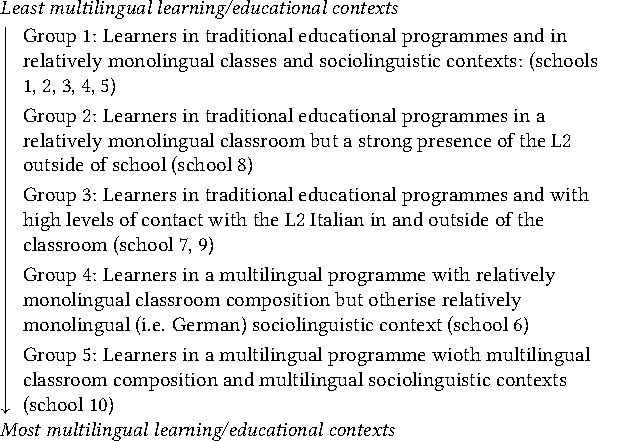
\includegraphics{figures/fig-7-1.pdf}
        \caption{Learning/educational context\label{fig:7:1}}
\end{figure}


As shown in \figref{fig:7:1}, the majority of schools are collocated at the less multilingual end of the continuum. Group 1, for example, comprises 5 schools, all providing subject teaching in L1 German and offering L2 Italian for 3--4 hours (from grade 2) and L3 English for 2 hours per week (from grade 4). In addition, pupils in group 1 live and study in relatively monolingual contexts with both the language constellation in their classrooms and the wider sociolinguistic surroundings being very homogeneous, i.e., Germanophone. 

Further down the continuum, contexts get more and more multilingual with some schools (groups 2 and 3) being located in areas where there is a high concentration of L2 (and/or other-language) speakers in the neighbourhood (NB: groups 2 and 3 differ from each other in terms of classroom composition and the wider sociolinguistic ecology). 

The school constituting group 4 is situated in a comparatively monolingual environment (see \figref{fig:7:2}) but purposely compensates for the demographics-related lack of contact with L2/n by providing for multilingual (cross-language and awareness-focused) learning within the school walls. 

Group 5 represents the most multilingual context with pupils studying in a distinctly multilingual classroom (both, in terms of the linguistic diversity of its student population and in terms of the teaching approach) and living in surroundings where L2 Italian and/or other languages are heard and spoken on a daily basis.

It is important to note that the two schools providing multilingual instruction, i.e. school 6 (= group 4) and school 10 (= group 5; see \figref{fig:7:2}) have a policy of fostering multilingualism and multiliteracy, which clearly qualifies them as multilingual schools \citep[32]{Cenoz2009}. School 10 (i.e., group 5) additionally provides for bilingual (German-Italian) literacy instruction from grade 1. In contrast to the distinct multilingual policy promoted by these schools, traditional or mainstream educational models do not (generally or overtly) aim at multilingualism and typically contend themselves with offering some (limited) L2 and L3 instruction. In these schools, promoting learners’ competency in L1 German tends to take priority over second and foreign language learning.

\figref{fig:7:2} further zooms in on the sociolinguistic and sociocultural contexts in which the schools are embedded. It shows that while some schools are located in areas (mostly small villages) with a mere 2\% of Italian speakers in the immediate surroundings, others (in larger towns) are situated in areas with a percentage of well over 70\% of Italian speakers. The percentages provided refer to the presence of Italian, German and Ladin speakers in the villages or towns in which the given schools are located. Again, the graph is intended to be read from top to bottom with the (relatively) monolingual contexts at the top end and the multilingual settings at the bottom end.

\begin{figure}[t]
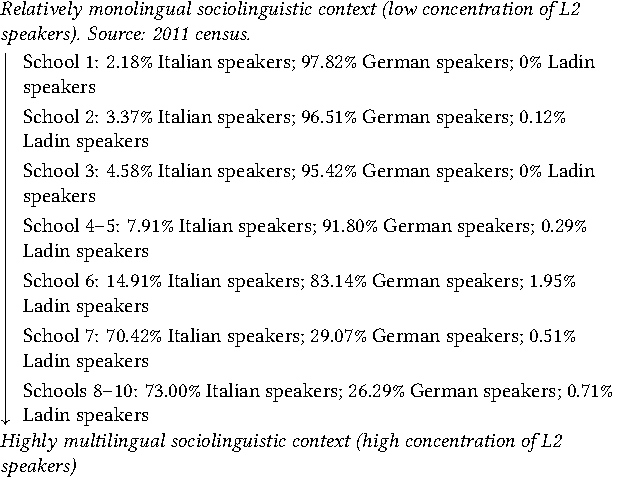
\includegraphics{figures/fig-7-2.pdf}
\caption{Sociolinguistic context\label{fig:7:2}}
\end{figure}


\largerpage
\subsection{Instruments and procedure}


To gain insight into young emergent multilinguals’ language-related attitudes and motivations, a questionnaire comprising a total of 26 items was administered (due to space restrictions, only 4 of these are discussed here). The questionnaire is divided into three sections, one focusing on language learning in general, one on learning L2 Italian and one on learning L3 English. The questionnaire was designed by the present author for the purposes of this research and probes into participants’ attitudes towards their L2 and L3, their perceptions relative to their own language learning experiences (in and outside of school), and relative to themselves as learners. In two open questions, the questionnaire further elicits children’s beliefs about the importance of learning Italian (L2) and English (L3), and about what they like best about learning languages.

The questionnaire was administered during school time under the supervision of the class teacher. Prior to administration, parents’ consent was obtained, and pupils and parents were informed about the aims of the study. Pupils were given 30 minutes to complete the questionnaire. Completion of the multi-item questionnaire required them to indicate (on a 4-point Likert-like scale) whether and to what extent they agree or disagree with statements such as:

\ea
\ea I think I am good at learning languages
\ex Learning languages comes easy to me
\ex I am afraid of making mistakes
\ex I like learning about other languages and cultures
\ex When I am older, I want to learn more languages
\ex I like learning Italian
\ex I like learning English
\ex I would like to be able to speak Italian really well one day
\ex I would like to be able to speak English really well one day 
\ex I like my Italian class
\ex I like my English class
\ex I think I am good at learning Italian
\ex I think I am good at learning English 
\ex My parents say that it is important to learn Italian
\ex My parents say that it is important to learn English 
\z
\z

In addition to completing the questionnaire, 42 pupils (recruited from 10\linebreak schools) took part in a short ten-minute interview in which they were asked questions about their use of strategies and how they learn languages. As part of the interview, children indicated with a smiling or stern face whether and how much they liked or disliked learning languages. In a second step, pupils then explained how their drawings were to be interpreted. 


% % % The pictures (\figref{fig:7:3}) provide a first glimpse of participants’ attitudes towards languages and language learning.    
% % % % \begin{figure}
% % % %   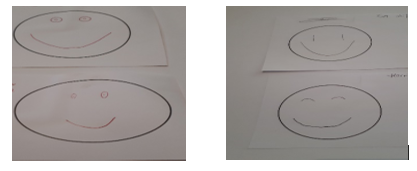
\includegraphics[width=\textwidth]{figures/fig-7-3.png}
% % % %   \caption{Children’s visualisations of their language (learning) attitudes (pictures taken by the author)\label{fig:7:3}}
% % % % \end{figure}


\largerpage
Interviews were semi-structured and were conducted during lesson time in a quiet part of the respective schools. Children were interviewed individually. Participation was voluntary. The working language was German. All interviews were digitally recorded, transcribed and coded according to thematic themes. 

For the qualitative evaluation, interviewees’ utterances were categorised as positive (+), negative (\textminus), or positive with some reservation ({\textasciitilde}). The overall score for comments was built cumulatively and is presented in \tabref{tab:7:5} (page~\pageref{tab:7:5}). 

In the following, I present first selective results relative to children’s attitudes to L2 Italian as obtained from the analysis of the questionnaires and interviews.

\largerpage
\subsection{Results}\label{sec:hofer:6.5}
\subsubsection{Quantitative findings}


The statistical analysis was performed utilising SPSS. Since the data are not normally distributed, the Kruskal-Wallis test as the non-parametric alternative to the one-way between-groups analysis of variance was used. To calculate the strength of the relationships between the variables, Kendall-Tau-b\slash Spearman correlations were applied. The significance level is 0.05.

While overall, pupils’ attitudes to L2 Italian are very positive (with 45.6\% of children stating that they like Italian very much, 49.3\% reporting they are very glad to be learning Italian, 61.6\% indicating they are highly motivated to study Italian, and 45.6\% declaring they very much like learning L2 in school), there are significant between-group differences as revealed by the Kruskal-Wallis test. The groups at the more monolingual end (i.e., groups 1 and 2) score significantly lower compared to the groups at the more multilingual end (groups 3, 4 and 5). Statistical differences obtained for pupils’ answers relative to their attitudes to learning Italian (“I like the Italian language”, $p = 0.038$; “I am glad to learn Italian”, $p = 0.034$; “I like learning Italian at school”, $p = 0.015$) and relative to their (LL) motivation (“I would like to know Italian really well, that's why I study a lot”, $p = 0.036$). The crosstabulations in the following detail the pertinent results according to groups. Results are organised around 4 items drawn from the questionnaire.

\begin{table}[b]
\begin{tabularx}{.8\textwidth}{YcSSSS}
\lsptoprule
      &     & \multicolumn{4}{c}{Answers (\%)}\\\cmidrule(lr){3-6}
Group & $n$ & {``No''} & {``A bit''} & {``A lot''} & {``Very much''}\\\midrule
1 & 98/101 & 1.0 & 18.2 & 42.4 & 38.4 \\
2 & 19/19  & 5.3 & 21.1 & 47.4 & 26.3 \\
3 & 54/55  & 3.7 & 11.1 & 27.8 & 57.4 \\
4 & 17/17  & 0.0 & 5.9 & 29.4 & 64.7 \\
5 & 15/15  & 0.0 & 13.3 & 33.3 & 53.3 \\
Total & 203/209 & 2.0 & 15.2 & 37.3 & 45.6\\\midrule
\multicolumn{6}{l}{$p = 0.016$, $r = 0.168$ (very weak effect)}\\
\lspbottomrule
\end{tabularx}
\caption{Crosstabulation attitudes: ``I like the Italian language''\label{tab:7:1}}
\end{table}


\begin{table}
\small
\begin{tabularx}{.8\textwidth}{YcSSSS}
\lsptoprule
      &     & \multicolumn{4}{c}{Answers (\%)}\\\cmidrule(lr){3-6}
Group & $n$ & {``No''} & {``A bit''} & {``A lot''} & {``Very much''}\\\midrule
1 & 98/101       & 1.0 & 13.3 & 40.8 & 44.9 \\
2 &  19/19       & 5.3 & 0.0 & 63.2 & 31.6 \\
3 &  54/55       & 0.0 & 11.1 & 38.9 & 50.0 \\
4 &  17/17       & 0.0 & 0.0 & 23.5 & 76.5 \\
5 &  15/15       & 0.0 & 0.0 & 33.3 & 66.7 \\
Total &  203/209 & 1.0 & 9.4 & 40.4 & 49.3 \\
\midrule
\multicolumn{6}{l}{$p = 0.015, r = 0.170$ (very weak effect)}\\
\multicolumn{6}{l}{Cramér’s V test: $p = 0.070, r = 0.181$ (very weak effect)}\\
\lspbottomrule
\end{tabularx}
\caption{Crosstabulation attitudes: ``I am glad to learn Italian''\label{tab:7:2}}
\end{table}

\largerpage
\tabref{tab:7:1} presents the results for participants’ response to the questionnaire item “I like the Italian language”. The Kruskal-Wallis test yielded a significant between-groups effect for this item at $p=0.016, r=0.168$ (very weak following Spearman). As can be gleaned from the percentages reported, the children in groups 3, 4 and 5 (positioned at the more multilingual end of the educational and/or sociolinguistic continuum) attained the highest scores at 57.4\%, 64.7\%, and 53.3\% respectively. No child in groups 4 and 5 reported not liking L2 Italian.  Groups 1 (38.4\%) and 2 (26.3\%) score significantly lower than the groups at the multilingual end.


\tabref{tab:7:2} reports the results for pupils’ answers to the item ``I am glad to learn Italian''. The Kruskal-Wallis test yielded a significant between-groups effect for this item at $p=0.015, r=0.170$ (very weak following Spearman). An additionally run Cramér’s V test revealed a sign. level of $p= 0.070, r= 0.181$ (very weak effect). Pupils in group 4 reach the highest score with 76.5\% indicating they are very glad to be studying Italian L2. At 66.7\%, the score for group 5 is the second highest. In group 3 the percentage is 50\%. No pupils in either of the three groups reports not being happy to learn Italian. Scores for groups 1 and 2 are significantly lower (44.9\% and 31.6\% respectively) than for groups 3, 4 and 5.


\begin{table}
\small
\begin{tabularx}{.8\textwidth}{YcSSSS}
\lsptoprule
      &     & \multicolumn{4}{c}{Answers (\%)}\\\cmidrule(lr){3-6}
Group & $n$ & {``No''} & {``A bit''} & {``A lot''} & {``Very much''}\\\midrule
1 & 98/101 & 1.0 & 13.3 & 29.6 & 56.1\\
2 &  19/19 & 5.3 & 0.0 & 57.9 & 36.8 \\
3 &  54/55 & 7.4 & 3.7 & 16.7 & 72.2 \\
4 &  17/17 & 0.0 & 0.0 & 17.6 & 82.4 \\
5 &  15/15 & 0.0 & 0.0 & 33.3 & 66.7 \\
Total   &  203/209 & 3.0 & 7.4 & 28.1 & 61.6 \\\midrule
\multicolumn{6}{l}{$p = 0.018, r = 0.165$ (very weak effect)}\\
\multicolumn{6}{l}{Cramér’s V: $p = 0.003, r = 0.220$ (weak effect)} \\
\lspbottomrule
\end{tabularx}
\caption{Crosstabulation attitudes: ``I would like to know Italian really well, that’s why I study a lot''\label{tab:7:3}}
\end{table}

\tabref{tab:7:3} provides the results of children’s answer to the questionnaire item “I would like to know Italian really well, that’s why I study…”. A significant effect was evinced at $p=0.018, r=0.165$ (very weak effect following Spearman). The additionally run Cramér’s V test revealed a sign. level of $p = 0.003, r = 0.220$ (weak effect). 82.4\% of pupils in group 4 reported a high level of motivation to improve their current level of L2. In group 5, the percentage is 66.7\%. With 72.2\% of pupils indicating they are working very hard to improve their L2, group 3 surpasses group 5 on this item. No child in groups 4 and 5 reports not wanting to work hard in order to improve their L2 proficiency. Scores for groups 1 and 2 are visibly lower (56.1\% and 36.8\%).


\begin{table}[b]
\small
\begin{tabularx}{.8\textwidth}{YcSSSS}
\lsptoprule
      &     & \multicolumn{4}{c}{Answers (\%)}\\\cmidrule(lr){3-6}
Group & $n$ & {``No''} & {``A bit''} & {``A lot''} & {``Very much''}\\\midrule
1 & 98/101 & 2.0 & 17.2 & 44.4 & 36.4\\
2 &  19/19 & 5.3 & 10.5 & 42.1 & 42.1\\
3 &  54/55 & 0.0 & 16.7 & 31.5 & 51.9\\
4 &  17/17 & 0.0 & 0.0 & 23.5 & 76.5 \\
5 &  15/15 & 0.0 & 0.0 & 46.7 & 53.3 \\
Total   &  203/209 & 1.5 & 13.7 & 39.2 & 45.6 \\\midrule
\multicolumn{6}{l}{$p = 0.002, r = 0.219$ (weak effect)}\\
\multicolumn{6}{l}{Cramér’s V: $p = 0.115, r = 0.172$ (very weak effect)}\\
\lspbottomrule
\end{tabularx}
\caption{Crosstabulation attitudes: ``I like learning Italian at school''\label{tab:7:4}}
\end{table}

\tabref{tab:7:4} shows the results for respondents’ reply to the item ``I like learning Italian at school''. A significant group effect was evidenced at $p=0.002, r=0.219$ (weak). Cramér’s V test indicates significance at $p = 0.115, r = 0.172$ (very weak effect). 76.5\% of children in group 4 report liking to learn L2 at school. The percentage for group 5 is 53.3\%, that for group 3 is 51.9\%. No pupil in any of the three groups reports not liking their L2 lessons. Groups 1 (36.4\%) and 2 (42.1\%) score much lower than the groups at the multilingual end. 

The ensuing section enlarges on the qualitative findings which serve as a complement to the statistical data.


\subsubsection{Qualitative findings}

As emerged from the interview data (and more specifically from children’s explanations of their drawings), pupils’ responses are overwhelmingly positive confirming the results yielded by the statistical evaluation of the questionnaires. Only a handful of children reported not enjoying language(s) learning (5 out of 42). It is indicative that it is only children in group 1 (the group at the more monolingual end) who express negative views about language(s) learning. Reasons therefor seem to be linked to the efforts required to build and maintain adequate or required proficiency levels in L2/L3 (see examples below). One is inclined to conjecture that participants in group 1 may be somewhat less conscious of the functional utility and personal enrichment of additional languages.

\begin{quote}\sloppy
\textit{Sprachen zu lernen gefällt mir nicht soo.} (NOESch)\\
`I don’t really like learning languages.'\medskip\\
\textit{Es ist halt schwierig Sprachen zu lernen, ja und in der Schule da ist das Sprachenlernen auch das anstrengendste.} (FELGr)\\
`Well, it’s difficult to learn languages, and in school it’s really hard work.'\medskip\\
\textit{Es ist vielleicht viel Arbeit […] Es gefällt mir nicht so gut.} (MIRISch)\\
`is perhaps hard work, don’t like it that much.'\medskip\\
\textit{Aber Sprachen lernen ist nicht so mein Ding.} (LUCIKna)\\
`learning languages is not really my cup of tea.'
\end{quote}

Most children, however, report enjoying languages and language(s) learning. As can be gleaned from the comments below, primary schoolers show a tendency to perceive languages as cool, fun, and exciting:

\begin{quote}
\textit{Weil ich die Sprachen toll finde.} (MOMBr)\\
`Because I think languages are great.'\medskip\\
\textit{Ich finde Sprachen sehr interessant, weil man auch etwas dazu lernt.} (STEFLei)\\
`I think languages are very interesting because you always learn something new.'\medskip\\
\textit{Sprachen sind cool.} (DAVSch)\\
`Languages are cool.'\medskip\\
\textit{Sprachen gefallen mir eigentlich gut, es sind viele neue tolle Wörter, besonders English, da muss man Wörter auch anders aussprechen, das gefällt mir.} (\mbox{LAURIZo})\\
`I quite like languages, there are many new and interesting words, especially in English, there you also have to pronounce words differently. I like that.'\medskip\\
\textit{… also Sprachenlernen find ich toll} (ROSTau)\\
`Language learning is cool'
\end{quote}

Pupils’ L(L) attitudes (as proffered in the course of the interviews) are summarised in \tabref{tab:7:1}. As can be seen from the figures adduced, the children in group 5 are the most positive about language(s) learning with all children in this group stating that they enjoy languages and language(s) learning. As for groups 2, 3, and 4, their attitudes are also predominantly positive with one child in each group, however, voicing reservations. Attitudinal patterns differ even more for group 1 where 5 children (out of 18) declare that they do not like language(s) learning and 5 more children express some degree of reservation (of the sort ``it’s hard work'', ``it requires a lot of effort'', etc.).

\begin{table}
\begin{tabular}{crccc}
\lsptoprule
Group & $n$ & \multicolumn{3}{c}{Attitudes}\\\cmidrule(lr){3-5}
      &     & + & \textminus & \textasciitilde\\\midrule                                             
1 & 18 & 8 & 5 & 5\\
2 & 3  & 2 & 0 & 1\\
3 & 10 & 9 & 0 & 1\\
4 & 7  & 6 & 0 & 1\\
5 & 4  & 4 & 0 & 0\\
\lspbottomrule
\end{tabular}
\caption{Language (learning) attitudes as reported in the individual interviews. +: positive; \textminus: negative; \textasciitilde: positive but with minor reservation\label{tab:7:5}}
\end{table}


\subsection{Discussion}


The present study examined the associations between sociolinguistic/learning context and young multilingual learner-users’ attitude to L2 Italian in South Tyrol. As a consequence of the specific demographics and spatial distribution of the linguistic groups, primary schoolers enrolled in German-language schools in South Tyrol may have different levels of exposure to Italian depending on whether they live in peripheral or more central locations. Accordingly, contact times differ substantially for children in remote rural villages vs the larger towns or capital. In addition, (language) education in mainstream versus multilingually-oriented classrooms can differ considerably. Following from these markedly differential initial (macro-level) conditions, it was hypothesised that pupils’ language learning experience reflects in their L(L) attitudes and motivation to learn Italian. This hypothesis is borne out by the quantitative and qualitative analysis. 

While overall, participants have been found to hold favourable attitudes towards L2 and L2 learning (thus confirming extant research in the field), a number of interesting findings have emerged from which equally interesting conclusions can be drawn. First, it is noteworthy that group 4 scored highest on all 4 items, i.e. they exhibit the highest level of positive attitudes towards Italian and the highest level of motivation to study it, surpassing even group 5 as the most multilingual cohort. On the learning continuum, group 4 is positioned at the more multilingual end. The children in this group benefit from a multilingual learning environment and a holistic integrative teaching approach, but the larger sociolinguistic ecology is relatively monolingual. This finding is somewhat unexpected. However, what we might infer therefrom is that even (comparatively) limited contact time within the framework of an integrated multilingual education programme can have significantly positive effects on young learner-users’ LL attitudes and motivation. 

Second, it is particularly worthy of consideration that group 3 overtakes group 5 (but not group 4) in the score for item 1 (``I would like to speak Italian really well, so I study Italian very much''). This may be linked to a perception among the children in group 3 that their level of proficiency does not match that of more competent (or native) Italian speakers in their immediate surroundings. Living in a highly multilingual environment (in and around the capital), the children in group 3 may have developed a certain awareness of the knowledge gap that separates them from more competent others, together with high expectations of themselves as learner-users of Italian. In addition, they may, owing to their distinctly multilingual life experience, be astutely aware of the necessity and benefits of mastering the language of their neighbours. Embedded as they are in a relatively monolingual lifeworld, pupils in group 4 may feel similar about the need to study hard in order to make headway in Italian (which may be why they scored highest on this item). On a purely speculative note, group 5 may be more confident about their Italian-language competency, which could be linked to their school’s holistic teaching approach, and acknowledgment of multilingual competences as by nature asymmetrical and domain-specific. Alternatively, it may also be the case that cohort 5 has come to adopt a more multilingual mindset which leads them to view their L2 competence from a resource-oriented rather than a deficit-oriented perspective.

Concluding, the main findings can be summarised as follows. As revealed by the quantitative analysis, pupils’ overall attitudes towards (learning) Italian are predominantly positive. The same holds for their motivated behaviour and their willingness to invest time and effort to improve their level of proficiency in Italian. The statistical results are in line with the findings yielded by the interview data. Overall, the outcomes of the current study then substantiate the findings reported by previous research which found a high appreciation for language(s) among young learners (\citealt{Nikolov1999}, \citealt{Shameem2004}). The results also reinforce the notion that important attitudinal benefits can accrue from early multilingual learning \citep{Helot2008}.

\section{Concluding remarks}

This paper has reported on work in progress. A selective review of the data set however allows for first important conclusions to be drawn. Overall language (learning) attitudes and motivation amongst the primary schoolers participating in the study turned out to be highly positive. Sociolinguistic and educational context, as it has been established, make a substantive difference in so far as children in more linguistically diverse settings with more exposure to L2 Italian hold more positive attitudes and are more motivated to expend time and effort to improve their L2 language skills. Based on the findings yielded, it can be concluded that type of early multilingual experience and amount of contact time with L2 (and/or other languages) do affect children’s LL attitudes and motivation. An important implication of this research is that formal multilingual learning programmes can act as attitudinal and/or motivational booster and thus compensate for lack of interactional opportunity in the immediate surroundings. Consonant with recent complexity- and dynamic systems-informed theorising and on the understanding that positive attitudinal patterns can be effected through multilingual instructional programmes, the present author calls for the wider implementation of multilingual models in South Tyrol (and beyond), with a vision to fostering not only learner-user attitudes and motivation (and ultimately learning outcomes), but also social cohesion and intercultural respect.

As for the larger research project underway, the next step will be to look into the intricate relations between contextual factors, learner attitudes and multilingual ability. Working within a dynamic systems\slash complexity theory framework, we do not anticipate simple straightforward cause-effect relationships but complex interdependencies and interactions between the multiple factors involved.

\section*{Abbreviations}
\label{sec:7:abbreviations}

\begin{tabularx}{.45\textwidth}{lQ}
YL  & Young learners\\
DMM & Dynamic model of  multilingualism\\
GLE & General language effort\\
LAE & Language acquisition effort\\
LME & Language maintenance effort\\
\end{tabularx}
\begin{tabularx}{.45\textwidth}{lQ}
EMM & Enhanced multilingual monitor\\
MLA & Metalinguistic abilities\\
XLA & Crossed linguistic abilities\\
CT  & Complexity theory\\
CLIL & Content and Language Integrated Learning\\
\end{tabularx}

{\sloppy\printbibliography[heading=subbibliography,notkeyword=this]}
\end{document}
